\section{Clinical and preclinical research: altered behavior in psychiatric conditions}

\subsection{Defining behavior}

Behavior is a fascinating and complex phenomenon which lies at the core of our existence as living organisms. The term refers to the manifestation of an individual's actions and reactions in response to external or internal stimuli, ultimately shaping interactions with the environment and other living things. Our understanding of behavior has evolved over time, and from a biological perspective, it encompasses an intricate interplay between genetic, neurobiological, and physiological processes \cite{Levitis2009BehaviouralBehaviour}.

To fully grasp the concept of behavior, it is essential to recognize the diverse nature of biological systems involved in its regulation. At the genetic level, heredity and individual variations in genetic makeup play a crucial role in shaping behavioral traits \cite{Charney2017GenesGenetics}. Genes can influence behavior through the expression of specific proteins, which in turn participate in the development, structure, and function of the nervous system \cite{Zhou2021Gene-EnvironmentPerspective}. While it is important to consider the impact of genetic factors, it is also necessary to acknowledge the interaction between genetics and environmental influences on behavior. This interplay, referred to as gene-environment interaction, highlights the dynamic nature of behavior and the continuous adaptation of living organisms to their surroundings \cite{Cuevas2019NeurotransmittersCycle}.

Moreover, a central component of behavior is the nervous system, responsible for receiving, processing, and transmitting information. It constitutes a highly organized network of specialized cells, such as neurons, which communicate with one another through complex electrochemical signaling, allowing for the integration and processing of sensory inputs, generation of responses, and modulation of behavior. Along these lines, neurotransmitters, the chemical messengers facilitating communication between neurons, also play a vital role in the regulation of behavior. These molecules, released by neurons, bind to specific receptors on the receiving cell, initiating a cascade of events that may either excite or inhibit the cell \cite{Luo2020PrinciplesNeurobiology}. 

Furthermore, another critical aspect of behavior is the interplay between the nervous and the endocrine systems. The latter is responsible for the production and release of hormones: chemical messengers secreted by endocrine glands that travel through the bloodstream and exert their effects on target cells \cite{Gardner2017GreenspansEdition}. Hormones can influence behavior by acting on the brain and other tissues, modulating emotions, mood, and stress responses \cite{McEwen2020HormonesScience}. Examples of hormones with significant impact on behavior include cortisol, which is involved in the stress response \cite{OConnor2020StressRisk}, and oxytocin, which plays a role in social bonding and attachment \cite{Bosch2018OxytocinDisruption}.

All in all, the delicate balance of neurotransmitters such as dopamine, serotonin, and glutamate, and hormones such as those mentioned above, is essential for maintaining normal behavioral functions. Disruptions in this balance can thus result in altered behavior, as seen in various psychiatric disorders \cite{AmericanPsychiatricAssociation2022DiagnosticDisorders}.

\subsection{A brief history of psychiatry}

The study of these altered behaviors, encompassed by the field of psychiatry, has a rich and storied history, marked by evolving theories and approaches to understanding and treating altered behavior in the context of mental health. The beginnings of psychiatry can be traced back to ancient civilizations, where mental disorders were often attributed to supernatural forces or divine intervention \cite{Fornaro2009MedicinePrejudices}. However, the modern understanding of psychiatry truly emerged during the Age of Enlightenment in the 18th century, when the focus shifted towards a more scientific and humane approach to mental health \cite{Kendler2022The1650-1850}.

One of the pioneers of this era was Philippe Pinel, a French physician who advocated for a compassionate approach to treating individuals with mental disorders. He emphasized the importance of understanding the root causes of altered behavior, paving the way for the development of modern psychiatric theories and therapies \cite{Wallace2008HistoryPsychology}. As psychiatry evolved throughout more recent periods of history, the field expanded its knowledge of the underlying biological processes influencing behavior, drawing upon the aforementioned discoveries in genetics, neurobiology, and endocrinology.

The 20th century marked significant advances in psychiatric research and treatment, driven by the emergence of psychoanalysis, behaviorism, and psychopharmacology. Sigmund Freud's psychoanalytic theory, which focused on unconscious processes and internal conflicts, had a profound impact on the understanding of human behavior \cite{Pick2015Psychoanalysis:Introduction}. Simultaneously, behaviorism, led by figures such as John Watson and B.\,F. Skinner, emphasized the role of observable behaviors and environmental influences in shaping human behavior \cite{Holland1978Behaviorism:Solution}. Psychopharmacology, the study of how drugs affect the mind and behavior, opened new avenues for treating psychiatric disorders by targeting the imbalances in neurotransmitters and hormones associated with them \cite{Rothschild2022Psychopharmacology:Basics}.

Despite the progress made in understanding and treating psychiatric disorders throughout history, however, challenges remain in fully elucidating the complex biological processes underlying altered behavior \cite{Harmer2017HowApproaches}. To address these challenges, researchers have increasingly turned to animal models as invaluable tools for studying the genetic, neurobiological, and physiological aspects of behavior \cite{Winship2019AnSchizophrenia, Varghese2017AutismModels, Wang2017TheDepression, Campos2013AnimalStress, Richter-Levin2019AnimalMet}. These models provide controlled environments in which researchers can manipulate specific factors, such as genetic mutations or environmental stressors, and measure their impact, typically in specific relevant variables \cite{Baker2020RodentPromises}.

Animal research has thus yielded essential insights into the neurobiology of psychiatric disorders, such as the role of neurotransmitter systems, neural circuitry, and genetic factors in the manifestation of altered behavior. For instance, rodent models have been crucial in understanding the role of dopamine in reward-related behaviors and addiction \cite{Wise2021DopamineAddiction}, as well as the involvement of serotonin in mood regulation and the pathophysiology of depression \cite{Borroto-Escuela2021TheProspects}. Additionally, animal models of stress have helped to elucidate the biological underpinnings of stress-related psychiatric disorders, such as anxiety and post-traumatic stress disorder (PTSD) \cite{Campos2013AnimalStress, Richter-Levin2019AnimalMet}. These findings highlight the importance of accurate behavioral quantification in understanding the etiology and progression of psychiatric disorders, as well as in the development of novel therapeutic strategies.

\subsection{Bridging the translational gap: from animal models back to humans}

While animal models have been instrumental in advancing the understanding of the neurobiology of psychiatric disorders, a translation gap persists when applying these findings to improve the lives of human patients. This gap arises from various factors, including differences in species, the complexity of human behavior, and the limitations of animal models in capturing the full spectrum of psychiatric symptoms \cite{Baker2020RodentPromises, Gururajan2019TheResearch}. In addition, the often fuzzy symptom-based definition of psychiatric disorders in humans makes it hard to disentangle unique biological mechanisms underlying disorders that fall into the same classification \cite{Miranda2021SystematicSubtyping}. Along these lines, initiatives such as the Research Domain Criteria (RDoC) have opened the field for discussion about more comprehensive, multimodal definitions of psychiatric disorders, which could have a positive impact in the future \cite{Vilar2019TranslationalRDoC}.

Thus, one of the primary challenges in bridging the aforementioned translation gap relates to the inherent differences between species. Although rodent models share some genetic, neurobiological, and physiological similarities with humans, there are significant differences in brain structure, function, and complexity. Consequently, the behavioral responses and underlying neurobiological mechanisms observed in animals may not fully mimic those in humans \cite{Bale2019TheDisorders}.

Moreover, human behavior is shaped by a multitude of factors, including culture, personal experiences, and social interactions \cite{Soderlund2018RelevanceNeuropsychiatry}. Animal models, although useful for studying basic biological processes, may not adequately capture the intricacies of human behavior and the unique environmental contexts that influence it. For instance, animal models of depression may rely on stress-induced behaviors, but these may not encompass the full range of cognitive and emotional symptoms experienced by humans with depression \cite{vonMucke-Heim2022IntroducingMice}.

Additionally, the validity of animal models in psychiatry depends on their ability to accurately mimic the clinical features of psychiatric disorders. While some animal models have been successful in recapitulating certain aspects of human disorders, they often do not cover the entire spectrum of symptoms or the heterogeneity observed in clinical populations. This limitation can hinder the development of effective treatments that address the diverse presentations of psychiatric conditions \cite{Baker2020RodentPromises, Soderlund2018RelevanceNeuropsychiatry}.

To minimize this translation gap, researchers are continuously refining animal models and developing new experimental paradigms that better reflect the complexity of human behavior and psychiatric symptoms. Along these lines, recent models, such as depression-like syndrome (DLS) in mice (Figure~\ref{fig:1.1}), leverage new technologies on comprehensive measuring to mix clinical criteria and RDoC to provide bio-behavioral reference syndromes for preclinical rodent models \cite{vonMucke-Heim2022IntroducingMice}.

In parallel, the evolution of behavioral quantification has played a pivotal role in advancing psychiatric research using both animal models and patients. From classical ethology to virtual reality and multi-modal tracking, the next sections explore the science behind translating such a complex phenomenon as behavior into meaningful quantitative variables.

\begin{figure}[!thb]
\centering
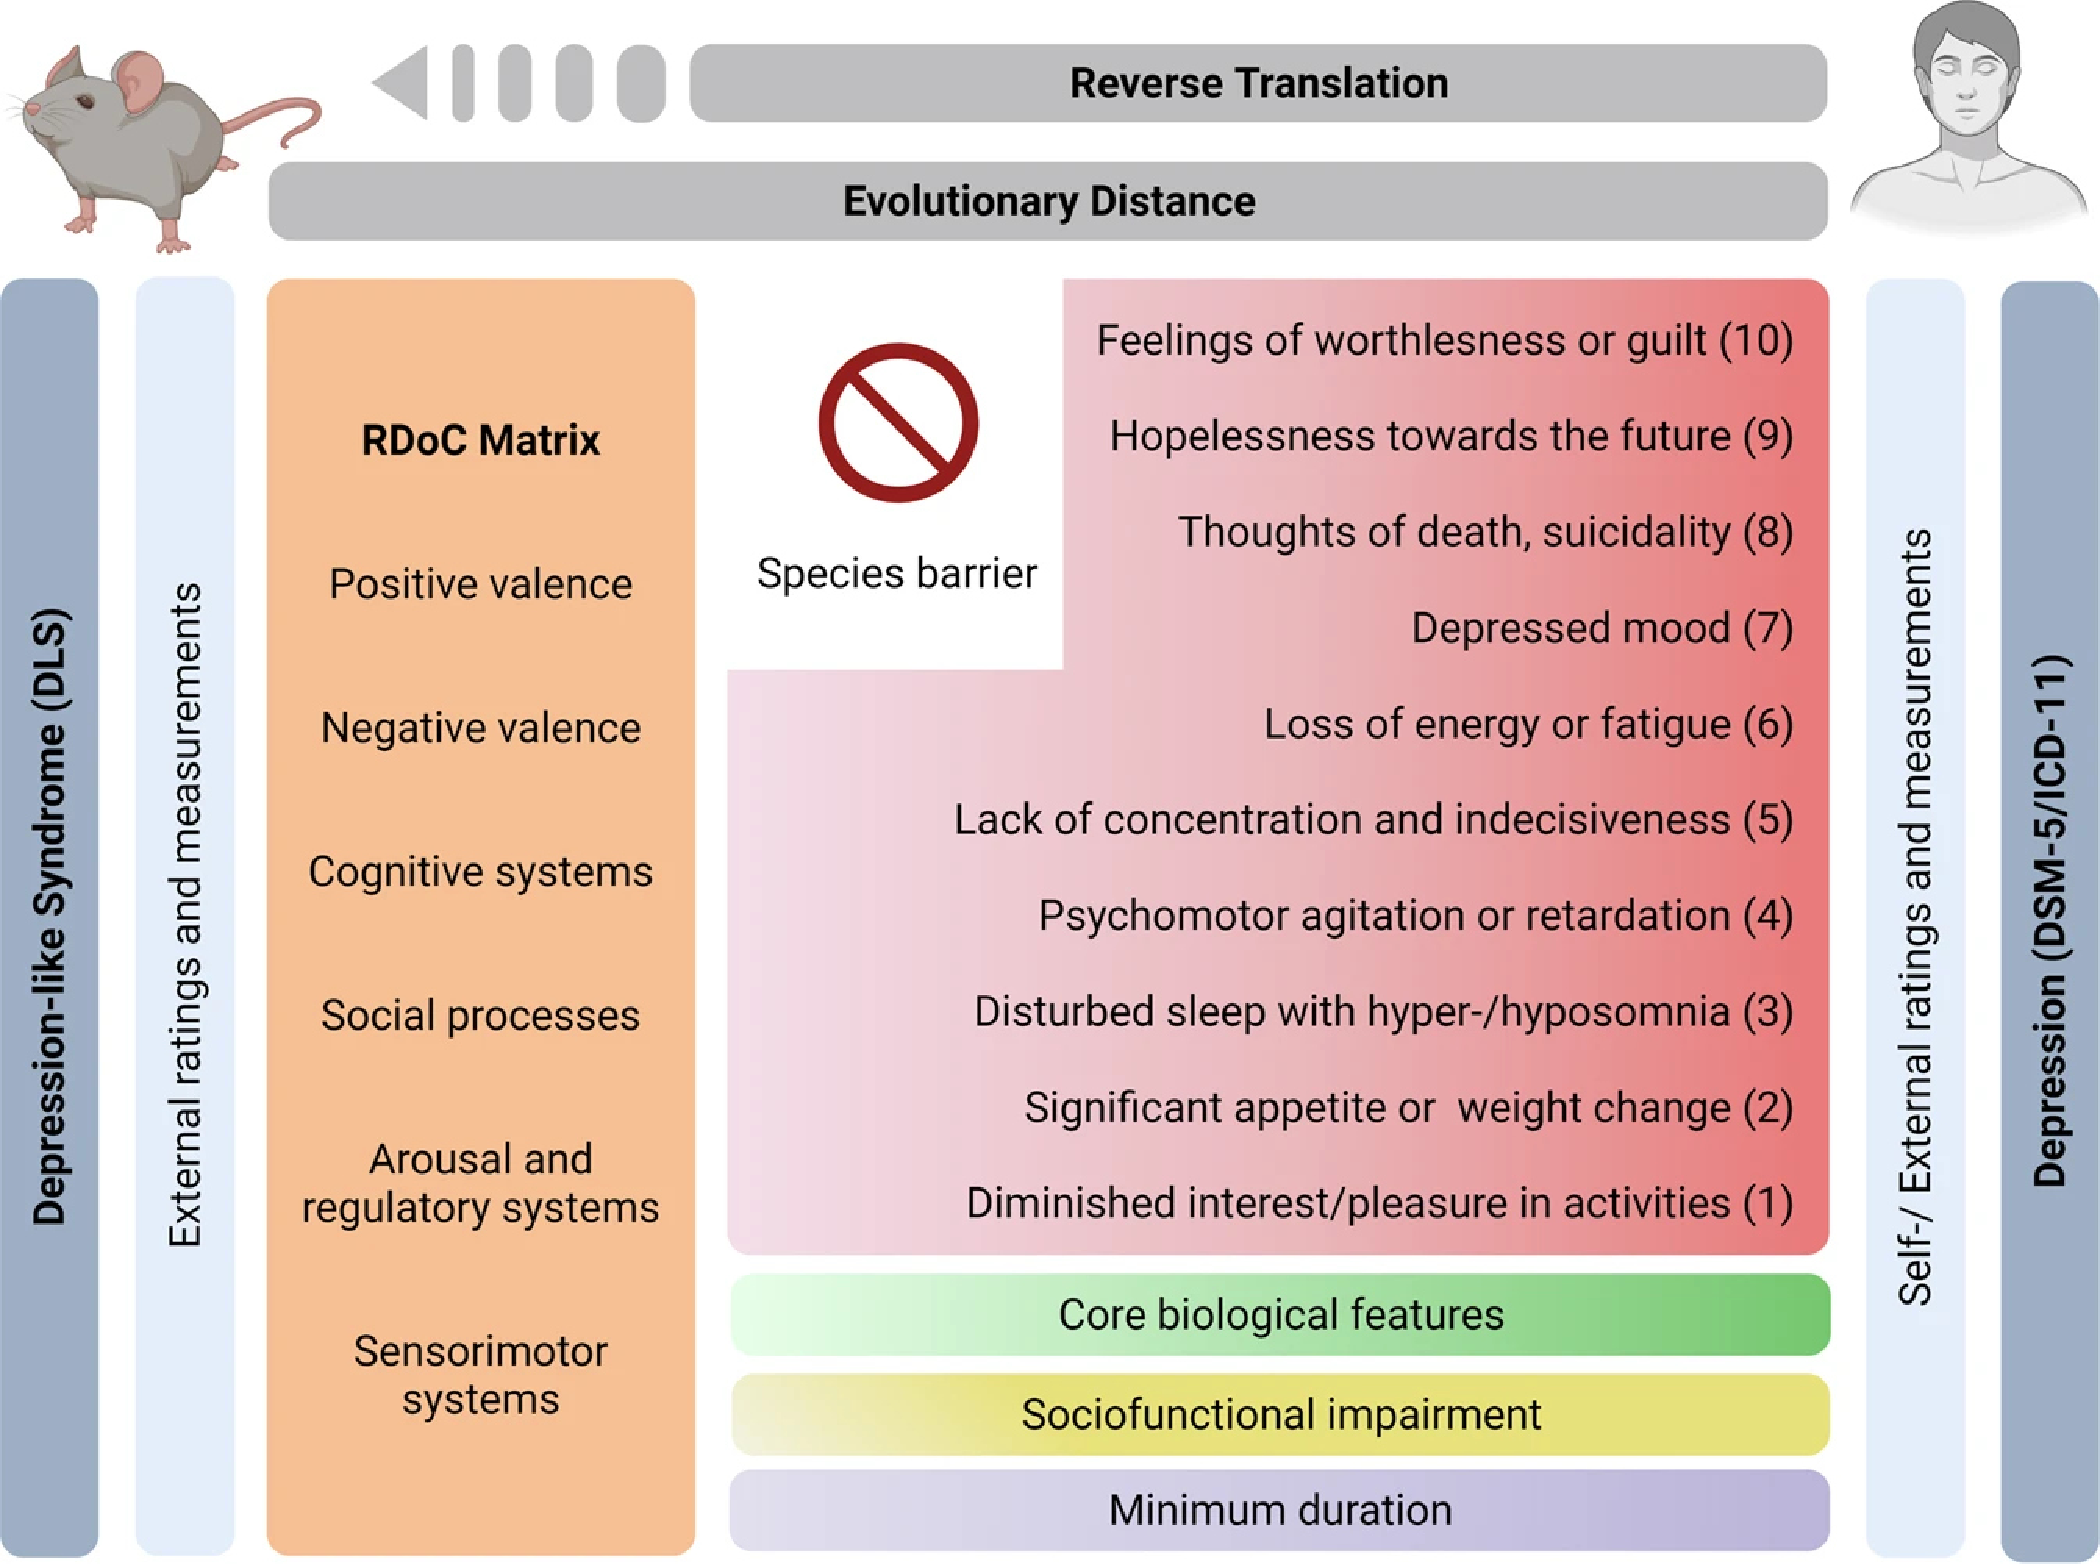
\includegraphics[width=\textwidth]{Figures/intro_1.pdf}

\caption[\textbf{Depression-like syndrome in mice}]{\textbf{Depression-like syndrome in mice:} Presented by von Mücke-Heim et al. in 2022, this model aims to bridge the gap between murine and human depression models. Beginning with the DSM/ICD definition of depression, the provided matrix illustrates the process of reverse translation, which takes criteria from human clinical settings and seeks to apply them to mice. There are, of course, certain symptoms of depression, such as feelings of worthlessness, that cannot be translated due to the evolutionary distance and species-specific barriers. However, many other symptoms, as well as key biological markers, socio-functional issues, and a certain minimum duration, can be effectively measured in mice. Examples of these include a decrease in appetite or significant weight loss. Both human and mouse measurements can then be sorted into RDoC domains. (Created with BioRender.com, adapted from \cite{vonMucke-Heim2022IntroducingMice}).}
\label{fig:1.1}

\end{figure}

\section{Quantifying behavior}

The field of animal behavior quantification has evolved considerably since its early days in the discipline of ethology. Pioneers such as Konrad Lorenz and Niko Tinbergen laid the foundation for systematic observations of animals in their natural environments, helping to establish fundamental principles and patterns of behavior \cite{Burkhardt2022Commentary:Ethology}. As the field progressed, researchers began to conduct controlled experiments in laboratory settings, allowing for more precise measurements and manipulations of experimental variables \cite{Scott1967ComparativeEthology}. These advancements in methodology provided valuable insights into the underlying mechanisms of animal behavior, which have in turn informed the development of novel technologies and computational techniques for quantifying and analyzing complex behavioral data \cite{Mathis2020APerspectives}.

\subsection{Endless forms most beautiful: from ethology to controlled behavioral experiments}

When the brain encounters external stimuli, it triggers specific patterns of cellular responses that ultimately shape behavioral outcomes. In the past, the foundational principles of behavior were typically derived from observational studies, where animals were left undisturbed in their natural environments \cite{Burkhardt2022Commentary:Ethology}. Early influential work in this area was carried out by Charles Darwin in the 19th century.
In his seminal work, ``On the Origin of Species" (1859) \cite{CharlesDarwin1859OnSpecies}, he introduced the concept of natural selection, which provided an explanation for the diverse array of shapes and behaviors observed in the animal kingdom. Moreover, his book ``The Expression of the Emotions in Man and Animals" (1872) \cite{CharlesDarwin1872TheAnimals} further delved into the subject, investigating the evolution and adaptive value of emotional expressions in both humans and animals. Thus, Darwin's work established a foundation for subsequent ethologists, arguably shaping the discipline's core principles. 

Thus and so, ethology was set to primarily work through observational methods, a core assumption of the discipline being that the most comprehensive understanding of behavior can be achieved by observing animals in natural or semi-natural environments. This approach allows researchers to study behavior descriptively, generating hypotheses and uncovering new behavioral concepts \cite{Marler2005EthologyEndocrinology}. A notable example of exceptional ethological achievement is the work led by Konrad Lorenz (1903--1989), an Austrian zoologist who is best known for his research on imprinting, a rapid learning process that occurs early in an animal's life, during which it forms strong attachments to certain stimuli. Through his work with greylag geese, Lorenz discovered that newly hatched goslings would imprint onto him, treating him as their parent. This observation revealed the innate nature of certain behavioral patterns, and emphasized the role of critical periods in the development of species-typical behaviors \cite{Sulloway1982DarwinLegend}. Along these lines, Niko Tinbergen (1907--1988), a Dutch biologist, set the grounds for a more comprehensive understanding of animal behavior with his ``four questions" framework, which is used to analyze animal behavior from four different perspectives: mechanism (or proximate causation), function (or ultimate causation), ontogeny, and phylogeny \cite{Burkhardt2016NikoArchives}. Ultimately, Tinbergen and Lorenz were awarded the Nobel Prize in Physiology or Medicine in 1973 (along with Karl von Frisch) for their discoveries concerning animal behavioral patterns.

While ethology and observational research have produced remarkable findings, however, there are significant limitations to these study designs. For instance, observational studies depend on the researcher's ability to accurately assess behavior, which can result in misinterpretation and differing interpretations among researchers. Additionally, the absence of control over environmental variables can lead to poorly reproducible results due, for example, to high variability between experimental conditions.

To address these limitations, the field of comparative psychology emerged, where researchers sought to uncover general principles of learning, cognition, and behavior within tightly controlled environments \cite{Scott1967ComparativeEthology}. The emphasis then shifted towards deconstructing the overall behavior into distinct, measurable elements, thus reducing its complexity through controlled laboratory settings, and enabling the isolation of the effects of specific factors on behavior (Figure~\ref{fig:1.2}). These lab tasks are characterized by their high degree of environmental control and standardized behavioral readouts, making causal inference and hypothesis-driven research questions possible \cite{Dettmer2021100Requires}. Pioneering researchers like Edward Thorndike, Ivan Pavlov, Burrhus Frederic Skinner, and others demonstrated the potential and power of this field. Along these lines, Thorndike illustrated the concept of trial-and-error learning by showing that animals became more efficient at escaping a device and obtaining rewards with an increasing number of trials \cite{Thorndike1898AnimalAnimals.}. Skinner, subsequently, developed one of the earliest and most popular laboratory behavioral tasks, the operant conditioning chamber (or ``Skinner box"), which can be used for both negative and positive reinforcement learning and still remains widely used in research \cite{Skinner1948SuperstitionPigeon}. This development initiated a trend to standardize and simplify various behavioral disciplines using laboratory tasks, a trend that continues to this day (Figure \ref{fig:1.3}). Laboratory tasks are of undeniable value for investigating the effects of external stimuli (e.\,g., the stress response system) and interventions (e.\,g., pharmacological) on behavior. Furthermore, the unparalleled possibilities of using various genetic mouse models have facilitated the study of specific target genes on behavior \cite{Baker2020RodentPromises}.

However, no behavioral tasks are flawless, and they carry assumptions and particular concerns that must be addressed. First and foremost, the general laboratory setups involve intensive interaction between the researcher and the test animals, raising concerns that inter-individual differences among researchers, such as sex, could impact the animals' behavioral performance \cite{Georgiou2022ExperimentersFactor, Chesler2002InfluencesBehavior, Sorge2014OlfactoryRodents}. Moreover, the current laboratory housing settings are highly unnatural, preventing rodents from engaging in species-typical behaviors and causing problematic behavior such as extreme aggression in group-housed animals \cite{Weber2017AggressionProblem}. Lastly, the use of inbred mice presents challenges when investigating naturalistic behaviors. Although genetic models have provided valuable insights into the genome, they have also resulted in animal models that behave quite differently from their wild counterparts, calling into question the validity of these models and, unfortunately, reducing the reproducibility of behavioral research \cite{Soderlund2018RelevanceNeuropsychiatry}.

All in all, taking a reductionist approach in laboratory tasks can be advantageous for many behavioral disciplines; however, it may also be detrimental for behavioral constructs that rely on multiple outputs and more naturalistic environments, making them more complex to evaluate. Recently, new technologies have enabled researchers to track animals in semi-naturalistic open-field settings in decreasingly invasive ways. By extracting reliable information from less restricted environments, experimenters can increase efficiency (by yielding multiple automatic read-outs per experiment) and explore more natural settings while retaining control over experimental variables (such as genetics or drug administration). Along these lines, the next section will delve into the computer science and machine learning (ML) advances that enabled this trend, and how they came to be.

\begin{figure}[!thb]
\centering
\includegraphics[width=\textwidth]{Figures/intro_2.pdf}

\caption[\textbf{From ethology to modern behavioral quantification}]{\textbf{From ethology to modern behavioral quantification:} The upper section of the figure depicts key methodologies used in behavioral neuroscience research, showing ethology on the left and comparative psychology on the right. The next generation of social behavioral tests, signified by the central arrow, utilize a semi-naturalistic environment. This combines the strengths of both ethology, providing a naturalistic setup free of experimenter interference, and comparative psychology, maintaining some level of environmental control by restricting space and external influences. Various elements, including exposure to stress, gender, motivation, recording duration, age-related changes, and living conditions, will have an impact on the results of the social behavioral evaluation. (Adapted from \cite{Bordes2023AdvancingLearning}).}
\label{fig:1.2}

\end{figure}

\begin{figure}[!thb]
\centering
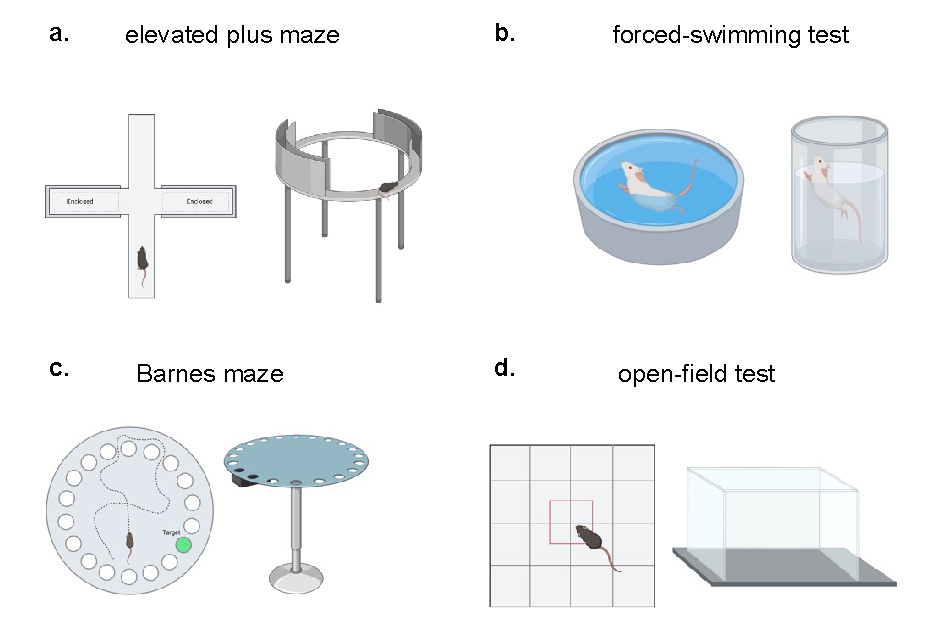
\includegraphics[width=\textwidth]{Figures/intro_3.pdf}

\caption[\textbf{Common univariate laboratory behavioral tasks}]{\textbf{Common univariate laboratory behavioral tasks:} \textbf{a.} Elevated plus mazes are commonly used setups to test for anxiety-like behavior. As anxious animals will tend to spend less time in the open arms, the ratio between time spent in open versus closed arms is typically reported. \textbf{b.} Forced-swimming tests are often used to measure anhedonic-like behavior, which is reported through helplessness time (the time the animals spend without trying to actively leave the pool where they are submerged). \textbf{c.}. Barnes' mazes are common tools to measure memory in rodents, where their ability to remember the location of specific target zones is tested. \textbf{d.} Open-field tests, typically used to assess locomotion, are becoming increasingly popular for automated feature extraction following pose estimation. (Created with BioRender.com).}
\label{fig:1.3}

\end{figure}

\subsection{Deep learning and the advent of markerless pose estimation}

The idea of tracking animals in more naturalistic experimental settings is not new. For example, in 2013 Shemesh et al. created an automatic phenotyping system based on video color recognition called the ``Social Box" \cite{Shemesh2013High-orderMice}. The authors described how social behavior in mice develops in a semi-natural environment, using techniques that quantify behavioral traits automatically, thus liberating researchers from laborious manual quantification. The authors automatically tracked several groups of mice in their home environment and investigated how individual behavior is strongly interdependent in their groups. In a follow-up study in 2019, Forkosh and colleagues developed a model, using the same system, that captures and outlines stable personality traits in mice \cite{Forkosh2019IdentityRepertoire}. While insightful, this work and subsequent studies were limited to tracking each animal's central position. Moreover, in these and other contemporary approaches, animal identification relied on dedicated (and often expensive or invasive) physical markers, such as radio frequency identifiers (RFID) or color hair dyes. Over the last decade, however, advancements in computer science, especially machine learning and deep learning-based computer vision, have sparked a revolution in animal motion tracking, enabling non-invasive markerless pose estimation of multiple body parts, which opened the floor for innumerable and creative ways of extracting behavioral information from more naturalistic (albeit controlled) environments.

To understand how this came to be, let us start from the beginning. Machine learning, a subfield within artificial intelligence (AI) which deals with methods that leverage data to improve computer performance on some set of tasks \cite{Roberts2021TheTheory}, arguably has its origins in the mid-20th century. One of the earliest proposed algorithms was the perceptron, introduced by Frank Rosenblatt in 1957 \cite{Rosenblatt1958TheBrain.}, which could be seen as a simple linear classifier that could learn to recognize patterns in data. Although limited in its capabilities, it laid the foundation for more advanced techniques, such as support vector machines and more complex neural networks. The 1980s subsequently marked the beginning of the modern era of machine learning with the emergence of decision trees, k-nearest neighbors (KNNs), and other algorithms that enabled computers to learn from data more effectively \cite{ChristopherMBishop2006PatternLearning}. Furthermore, the development of the backpropagation algorithm by Geoffrey Hinton and his colleagues in 1986 allowed for more efficient training of neural networks, setting the stage for the rise of deep learning \cite{Rumelhart1986LearningErrors}.

Deep learning is born then as a subfield of machine learning, which involves the use of artificial neural networks (ANNs) with multiple hidden layers to learn complex, hierarchical representations of data \cite{Roberts2021TheTheory}. The first breakthrough of deep learning arguably came in 2012 when Alex Krizhevsky, Ilya Sutskever, and Geoffrey Hinton developed AlexNet, a deep convolutional neural network (CNN) that significantly outperformed other methods in the ImageNet Large Scale Visual Recognition Challenge \cite{Krizhevsky2012ImageNetNetworks}. This success marked the beginning of the ``deep learning revolution" and led to rapid advancements in various AI applications, including computer vision, natural language processing, and speech recognition. In computer vision in particular, deep learning enabled the departure from hand-crafted feature extraction methods popular in since the 1960s, which proved to be insufficient for complex, real-world tasks \cite{Chai2021DeepScenarios}. Since then, there have been numerous breakthroughs, including Faster R-CNN for object detection \cite{Ren2015FasterNetworks}, Generative Adversarial Networks (GANs) and diffusion models for image synthesis \cite{Gui2020AApplications, Rombach2021High-ResolutionModels}, and the introduction of the Transformer architecture, which has further enhanced the capabilities of natural language processing and computer vision systems \cite{Dosovitskiy2020AnScale}, among others. Moreover, the development of increasingly performant models for multi-class image classification led to the rise of effective transfer learning, where models that had been pre-trained in large datasets, such as ImageNet, can be used for feature extraction, and fine-tuned or repurposed altogether for a different downstream task, without the need for full retraining \cite{Iman2022AAdvancements}.

It is in this context that tools like DeepLabCut \cite{Mathis2018DeepLabCut:Learning}, SLEAP \cite{Pereira2022SLEAP:Tracking}, and SIPEC \cite{Marks2022Deep-learning-basedEnvironments}, were developed in the last few years. By leveraging deep neural networks (DNNs) pre-trained in ImageNet, base versions of these models are capable of detecting the position of a set of user-defined body parts in each frame of a given video dataset, upon fine-tuning with very little human labelling. While several architectures have been developed to date, the basic idea consists of replacing the classification layers of a chosen pre-trained model (typically ResNet50 \cite{He2015DeepRecognition}) with deconvolutional layers that output a probability mass map for each body part, and each pixel on the original image (Figure~\ref{fig:1.4}). Furthermore, the $argmax$ of the output for each body part can then be interpreted as a confidence value, enabling further downstream filtering or processing of defective tracks. The incorporation of deep learning techniques into animal motion tracking has not only simplified the data collection process, but also improved the quality and granularity of the information gathered, providing researchers with unparalleled opportunities to investigate intricate behavioral patterns and their underlying neural mechanisms, both while retaining control on experimental variables and in the wild \cite{Tuia2022PerspectivesConservation}.

In this fashion, these approaches have made it possible to gather vast amounts of time series data on multiple body parts with human-level accuracy \cite{Sturman2020DeepSolutions}. Additionally, some models can now retain individual identification in social settings without dedicated hardware, making it possible to track multiple animals at once, which paves the way for social behavioral analysis \cite{Pereira2022SLEAP:Tracking, Lauer2022Multi-animalDeepLabCut}. 

Moreover, and in contrast to instances where experimental breakthroughs have triggered an increase in data volume (thereby sparking the need for new computational approaches) the case of behavioral analysis has followed the opposite trend \cite{Miranda2023IncreasingBehaviors}. Here, the deliberate application of recent computational techniques has led to a rapid increase in data collection, enabling even more technical breakthroughs (such as foundation models for particular species \cite{Ye2022SuperAnimalBehavior}), and ultimately changing how research is conducted and the types of questions people can ask \cite{Mathis2020APerspectives}. In the next section, we discuss how precision tracking data can be analyzed, to gain new insights into animal behavior and answer scientific questions that were much harder to address before this field came to be.

\begin{figure}[!thb]
\centering
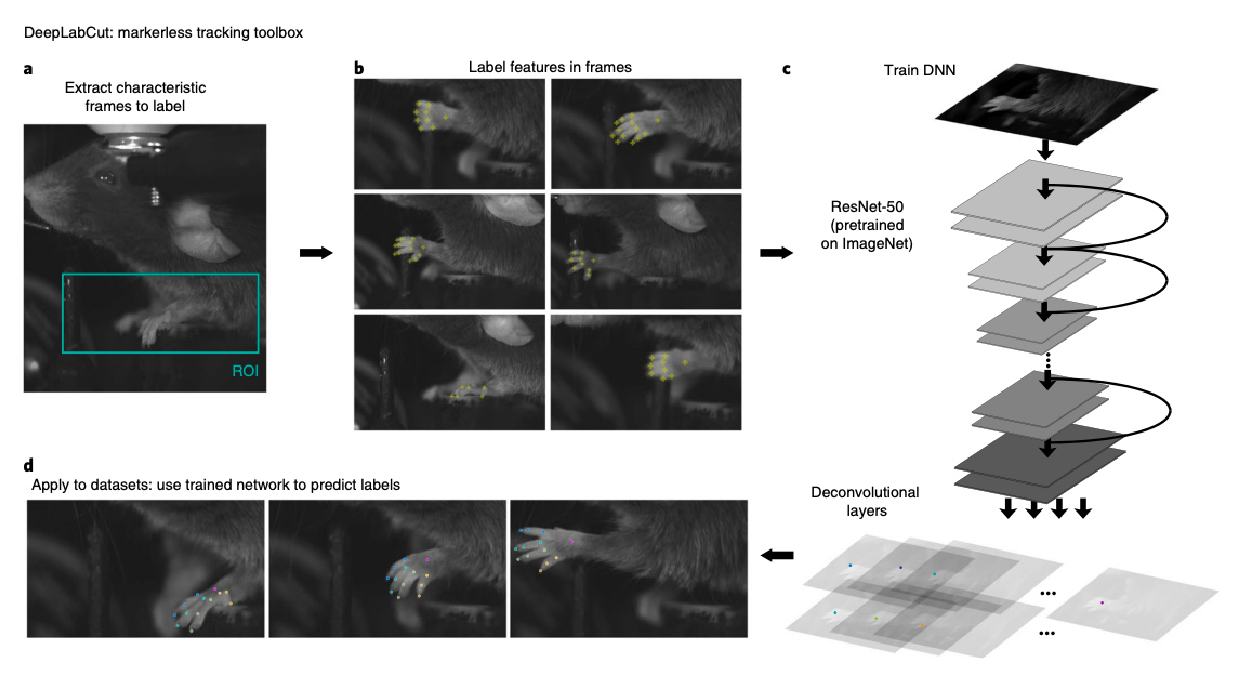
\includegraphics[width=\textwidth]{Figures/intro_4.pdf}

\caption[\textbf{DeepLabCut overview:} novel algorithms for markerless motion tracking]{\textbf{DeepLabCut overview:} \textbf{a.} The process begins with the extraction of images displaying distinct postures that are representative of the specific animal behavior. To enhance computational efficiency, the region of interest (ROI) should be minimized, while still encompassing the behavior under study, which in this case is reaching. \textbf{b.} Next, the user is required to manually identify and label various body parts. In this context, different joints of the digits and the wrist were pinpointed as features of interest. \textbf{c.} A deep neural network (DNN) architecture is then trained to predict the locations of the labeled body parts based on the associated image. A unique readout layer is produced for each body part, designed to predict the likelihood of a body part appearing in a specific pixel. Training adjusts the readout and DNN weights, which are stored post-training. \textbf{d.} The trained network can then be utilized to determine the positions of the body parts from video footage. The images depict the most probable locations for the 13 labeled body parts on a mouse's hand. (Adapted from \cite{Mathis2018DeepLabCut:Learning}).}
\label{fig:1.4}

\end{figure}

\section{Automated annotation of motion tracking data}

As previously discussed, deep learning based pose estimation made a strong impact in the amount of information that can be extracted from raw animal experiment video. In this section, we will explore the plethora of methods that became available to annotate, analyze, and ultimately extract meaning from this novel and rich paradigm. These methods will be mostly described as falling into one of two big families, namely supervised classification (aiming to extract pre-determined and characterized traits) and unsupervised embedding and clustering (seeking to explore data and extract patterns without explicit external input). Combinations between the two, such as clustering-powered active learning platforms, will also be touched upon.

\subsection{Supervised annotation}

Either by observational research or as the result of controlled experiments, behavioral neuroscience has had time to develop and describe detailed ethograms for specific animal models \cite{deChaumont2019Real-timeLearning}. That is, descriptions of typical actions these experimental animals conduct in the environments in which they are typically observed. The supervised annotation of motion tracking time series, then, aims to use classification models to detect, upon being fed with labelled examples, the moments in time where animals perform certain actions, that may or may not be related to a specific experimental condition. 

Along these lines, a current common-use package that requires minimal coding to create supervised behaviors from DLC and other pose-estimation packages is SimBA (Simple Behavioral Analysis \cite{Ro2020SimpleAnimals}). SimBA enables users to label behaviors of interest in a graphical user interface, training machine learning models that can learn the rules underlying certain behaviors directly from data, thus automating the quantification of arbitrarily complex traits. Moreover, the provided models (typically ensemble classifiers such as Gradient Boosting Machines---GBMs) are trained on extracted static and dynamic features describing animal motion, rather than the sequences themselves \cite{Burns2018Seglearn:Series}. This approach makes the models lighter to train and doesn't require a dedicated graphics processing unit (GPU). Additionally, certain packages, such as the previously mentioned SIPEC \cite{Marks2022Deep-learning-basedEnvironments} or MARS \cite{Segalin2021TheMice}, integrate a custom tracking system with a supervised behavioral annotation pipeline, offering benefits over combining different packages for the same purpose since users do not need to worry about software compatibility within different frameworks. 

All these approaches work very well at detecting previously defined patterns. However, their generalizability across behavioral setups is rather limited for complex behaviors, forcing users to relabel data and retrain models almost every time a new dataset comes along. Nonetheless, some behaviors can be accurately reduced to a set of hard-coded rules, without the need for model training \cite{Shultz2017CurseDimensionality}. These include, but are not limited to, time-in-zone quantification, specific individual interactions (e.\,g., nose to nose and nose to tail contacts), or interactions with objects. Simple approaches in this case can help reduce overfitting in some very relevant scenarios \cite{Bordes2023AutomaticallyStress}. Moreover and leaving generalizability issues aside, while supervised classification models can drastically increase annotation throughput when compared to classical univariate behavioral tasks, they are still restricted to a set of pre-defined and labelled patterns. This can result in leaving out meaningful yet undescribed animal behaviors, which could be better captured with a different set of methods.

\subsection{Unsupervised annotation and behavioral embeddings}

An alternative approach to annotating behavior involves analyzing pose-estimation data without pre-established ethograms. This can be achieved through unsupervised learning techniques, a branch of machine learning that seeks to extract insights from data without prior information about the outcomes of interest \cite{ChristopherMBishop2006PatternLearning}. 

By retrieving behavioral clusters or syllables expressed at particular points in time, unsupervised algorithms in this context have the potential to help create automatic comprehensive ethograms, bypassing the limitations of the previously described classification methods, and hinting by themselves at new knowledge \cite{Weinreb2023Keypoint-MoSeq:Dynamics}.

Additionally, these approaches facilitate hypothesis generation, as they can identify behavioral patterns indicative of previously unknown behaviors within a specific context. Since unsupervised methods allow for exploration of the behavioral space without the need for labeling, they can serve as an initial screening for behaviors of interest. For instance, clustering can be employed to pinpoint at particular behavioral patterns displaying the most significant differences between predefined experimental conditions \cite{Bordes2023AutomaticallyStress}. Subsequently, researchers can train supervised classifiers to more directly and accurately measure the behaviors of interest. In this regard, new approaches have been published recently in which unsupervised clusters are used to initialize supervised classifiers, which are in turn fine-tuned using an active learning framework \cite{Schweihoff2022A-SOiDBehavior}.

Along these lines, several packages and pipelines have been developed that automatically segment behavior using unsupervised methods. For example, the software system B-SOiD \cite{Hsu2021B-SOiDBehaviors} annotates motion data with feature sets that help describe behavior over time without directly using sequential data. Another software system, MoSeq \cite{Weinreb2023Keypoint-MoSeq:Dynamics, Wiltschko2020RevealingSequencing}, leverages the time component of motion with autoregressive hidden Markov models, which can directly capture probabilistic relationships between input variables. Other packages, like VAME \cite{Luxem2022IdentifyingMotion}, employ neural networks that process motion sequences directly, and apply post-hoc clustering techniques on the resulting latent space, yielding more meaningful clusters of specific behaviors with less noise from other patterns \cite{Rubio2023Auto-EncodersPerspectives}. Thus and so, an added benefit of neural network models is their ability to embed motion trajectories into interpretable latent spaces that can be, for example, analyzed differentially across experimental conditions \cite{Bordes2023AutomaticallyStress}. Moreover, understanding the retrieved patterns is crucial for comprehending the underlying behaviors. The ability to interpret the models' outputs can not only enhance transferability across datasets in the case of supervised learning, but also aid the meaningful interpretation of unsupervised clusters. In this context, both visual exploration (taking advantage of video data and mapping back to snippets assigned to specific patterns) and machine learning explainability tools, such as Shapley Additive Explanations (SHAP) \cite{Goodwin2022TowardNeuroscience}, are suitable approaches.

\begin{figure}[H]
\centering
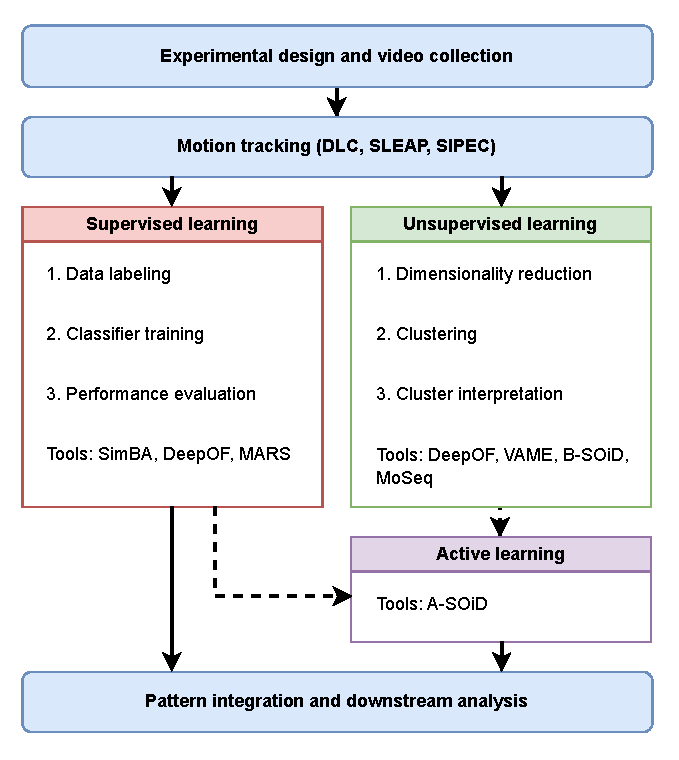
\includegraphics[width=(\textwidth - 85pt)]{Figures/intro_5.pdf}

\caption[\textbf{Automatic behavioral annotation via motion tracking:} exploring different annotation options]{\textbf{Automatic behavioral annotation via motion tracking:} Once the experimental design is established and videos are gathered, keypoints from one or multiple animals are extracted over time as time series, using tools like DeepLabCut, SLEAP, or SIPEC. Predetermined behaviors can be identified with supervised learning tools such as SimBA, or MARS, which typically require data labeling, classifier training, and an evaluation of the performance of the extracted behaviors. However, tools like DeepOF offer pre-trained models, eliminating these steps. An alternative method for obtaining a wider scope of information is through unsupervised learning, which doesn't require labeling, and aims to derive behavioral syllables or clusters following a dimensionality reduction step. The interpretation of these clusters is also a crucial step, which can be done via visual video inspection or using model explainability techniques like SHAP. This category includes tools such as DeepOF, VAME, B-SOiD, and MoSeq, to name a few. In addition, the results from unsupervised learning can serve as a starting point for supervised models with active human feedback, as demonstrated in the A-SOiD framework. Lastly, the expression and dynamics of all acquired patterns can be compared across different experimental conditions to gain insights into behavioral changes. (Adapted from \cite{Bordes2023AdvancingLearning}).}
\label{fig:1.5}

\end{figure}

In summary, the use of supervised and unsupervised methods in automated behavioral analysis is key to leverage new tracking technologies, and holds the potential to significantly contribute to our understanding of animal behavior in the near future, revealing new patterns and helping to streamline research efforts. New and innovative methods that can help analyze these data in meaningful ways can thus positively impact the current state of the field. An overview of this pipeline can be found in figure~\ref{fig:1.5}.

The next section of this introduction will delve into the fundamental biology and behavioral implications of chronic stress, which serves as the case study for applying the algorithms and analyses developed in this thesis.

\section{Chronic stress as a case study}

Chronic stress serves as an ideal illustration of the complex connections between animal behavior and psychiatric disorders. It has been associated with the development or worsening of numerous psychiatric conditions, including major depressive disorder (MDD), post-traumatic stress disorder (PTSD), anxiety disorders, and even neurodegenerative diseases like Alzheimer's and Parkinson's \cite{Sanacora2021TheDisorders}. In animal models, chronic stress exposure can lead to behavioral changes similar to those observed in human patients, such as heightened anxiety-like behavior, cognitive impairments, and disruptions in social interactions \cite{Musazzi2016TheDisorders, Davis2017NeurobiologyStudies, Musazzi2018WhatDisorders}. Examining the effects of stress on animal behavior has not only deepened our understanding of the intricate relationship between stress and psychiatric disorders but has also provided insights into underlying neurobiological mechanisms and potential therapeutic interventions. In this section, we explore the basic biology behind stress, and the Chronic Social Defeat Stress (CSDS) model in mice, which will serve as a case study for the models presented in this thesis.

\subsection{A primer on stress biology}

Stress is an integral part of our daily lives, affecting our mood and motivation. Biologically speaking, it refers to the body's response to external or internal stimuli that challenge its equilibrium, known as stressors. This response involves the complex interplay of neural and endocrine structures to help the organism adapt to particularly demanding situations. Along these lines, central to the stress response is the activation of the hypothalamic-pituitary-adrenal (HPA) axis, which leads to the release of cortisol, a hormone central to energy, blood pressure, and mood regulation. As a consequence, the sympathetic nervous system (SNS) is activated, resulting in the secretion of catecholamines, such as adrenaline and noradrenaline, from the adrenal medulla \cite{Godoy2018AImplications}. These neuroendocrine changes prepare the body for the ``fight or flight" response, a concept introduced by Walter Cannon to describe the physiological adaptations that enable an individual to confront or evade a perceived threat \cite{Cannon1953BodilyExcitement.}. This response includes increased heart rate, blood pressure, and respiration, as well as heightened alertness and the mobilization of energy resources. While short-term activation of the stress response can be beneficial for survival, chronic stress can lead to detrimental effects on physical and mental health, highlighting the significance of understanding the biological mechanisms underlying its regulation \cite{Davis2017NeurobiologyStudies}.

Notably, chronic stress has increasingly become a societal burden, with the incidence of stress-related disorders steadily growing over the past decades \cite{WorldHealthOrganization2021DepressionEstimates}. Furthermore, our understanding of the behavioral and neurobiological mechanisms related to these disorders is limited, which contributes to the moderate success of current drug treatments \cite{Shemesh2023ANeuroethology}. Furthermore, the adopted symptom-based classification of these disorders, and the resulting heterogeneity, makes it often difficult to uncover their potential common biological causes \cite{Crocq2015ADSM, Miranda2021SystematicSubtyping}.

Along these lines, deciphering the complexity of neurobiological circuits and molecular pathways underlying healthy or abnormal stress responses requires the integration of cellular, molecular, and behavioral data \cite{Miranda2023IncreasingBehaviors} (Figure~\ref{fig:1.6}). While traditional approaches may lack the necessary spatial and temporal resolution, recent technological advancements have considerably improved these aspects. For example, single-cell transcriptomics enabled the investigation of thousands of genes simultaneously and the dissection of the contributions of different cell types involved in the stress response \cite{Lopez2021Single-cellAdaptation}. Similarly, the use of activity-dependent labeling methods combined with brain-clearing techniques allows for the identification of activated cells following specific stressors and the reconstruction of the involved brain circuits in a particular stress response \cite{Li2020ComputationalCentury}. As with most high-throughput techniques, these strategies generate vast amounts of data, necessitating the use of appropriate computational and statistical tools. Consequently, advancements in molecular and cellular neuroscience techniques have spurred growth in computational science and the development of suitable data analysis software. This way, the previously discussed novelties in behavioral phenotyping have also enabled researchers to efficiently assess the specific effects of different types of stressors, stress paradigms, developmental ages, and sex on behavior, while significantly reducing manual scoring-related bias \cite{Shemesh2023ANeuroethology}. Moreover, advances in virtual reality (VR) have also allowed researchers to test therapies and track behavioral responses in human patients \cite{Binder2020QuantifyingReality, Binder2022FacingPhobia}.

Furthermore, and as previously discussed, to understand the cellular and molecular mechanisms responsible for the pathophysiology of psychiatric disorders, it is crucial to develop and implement preclinical animal models. A common model used in current neurobiological research, namely Chronic Social Defeat Stress (CSDS) is presented in the next section.

\begin{figure}[!thb]
\centering
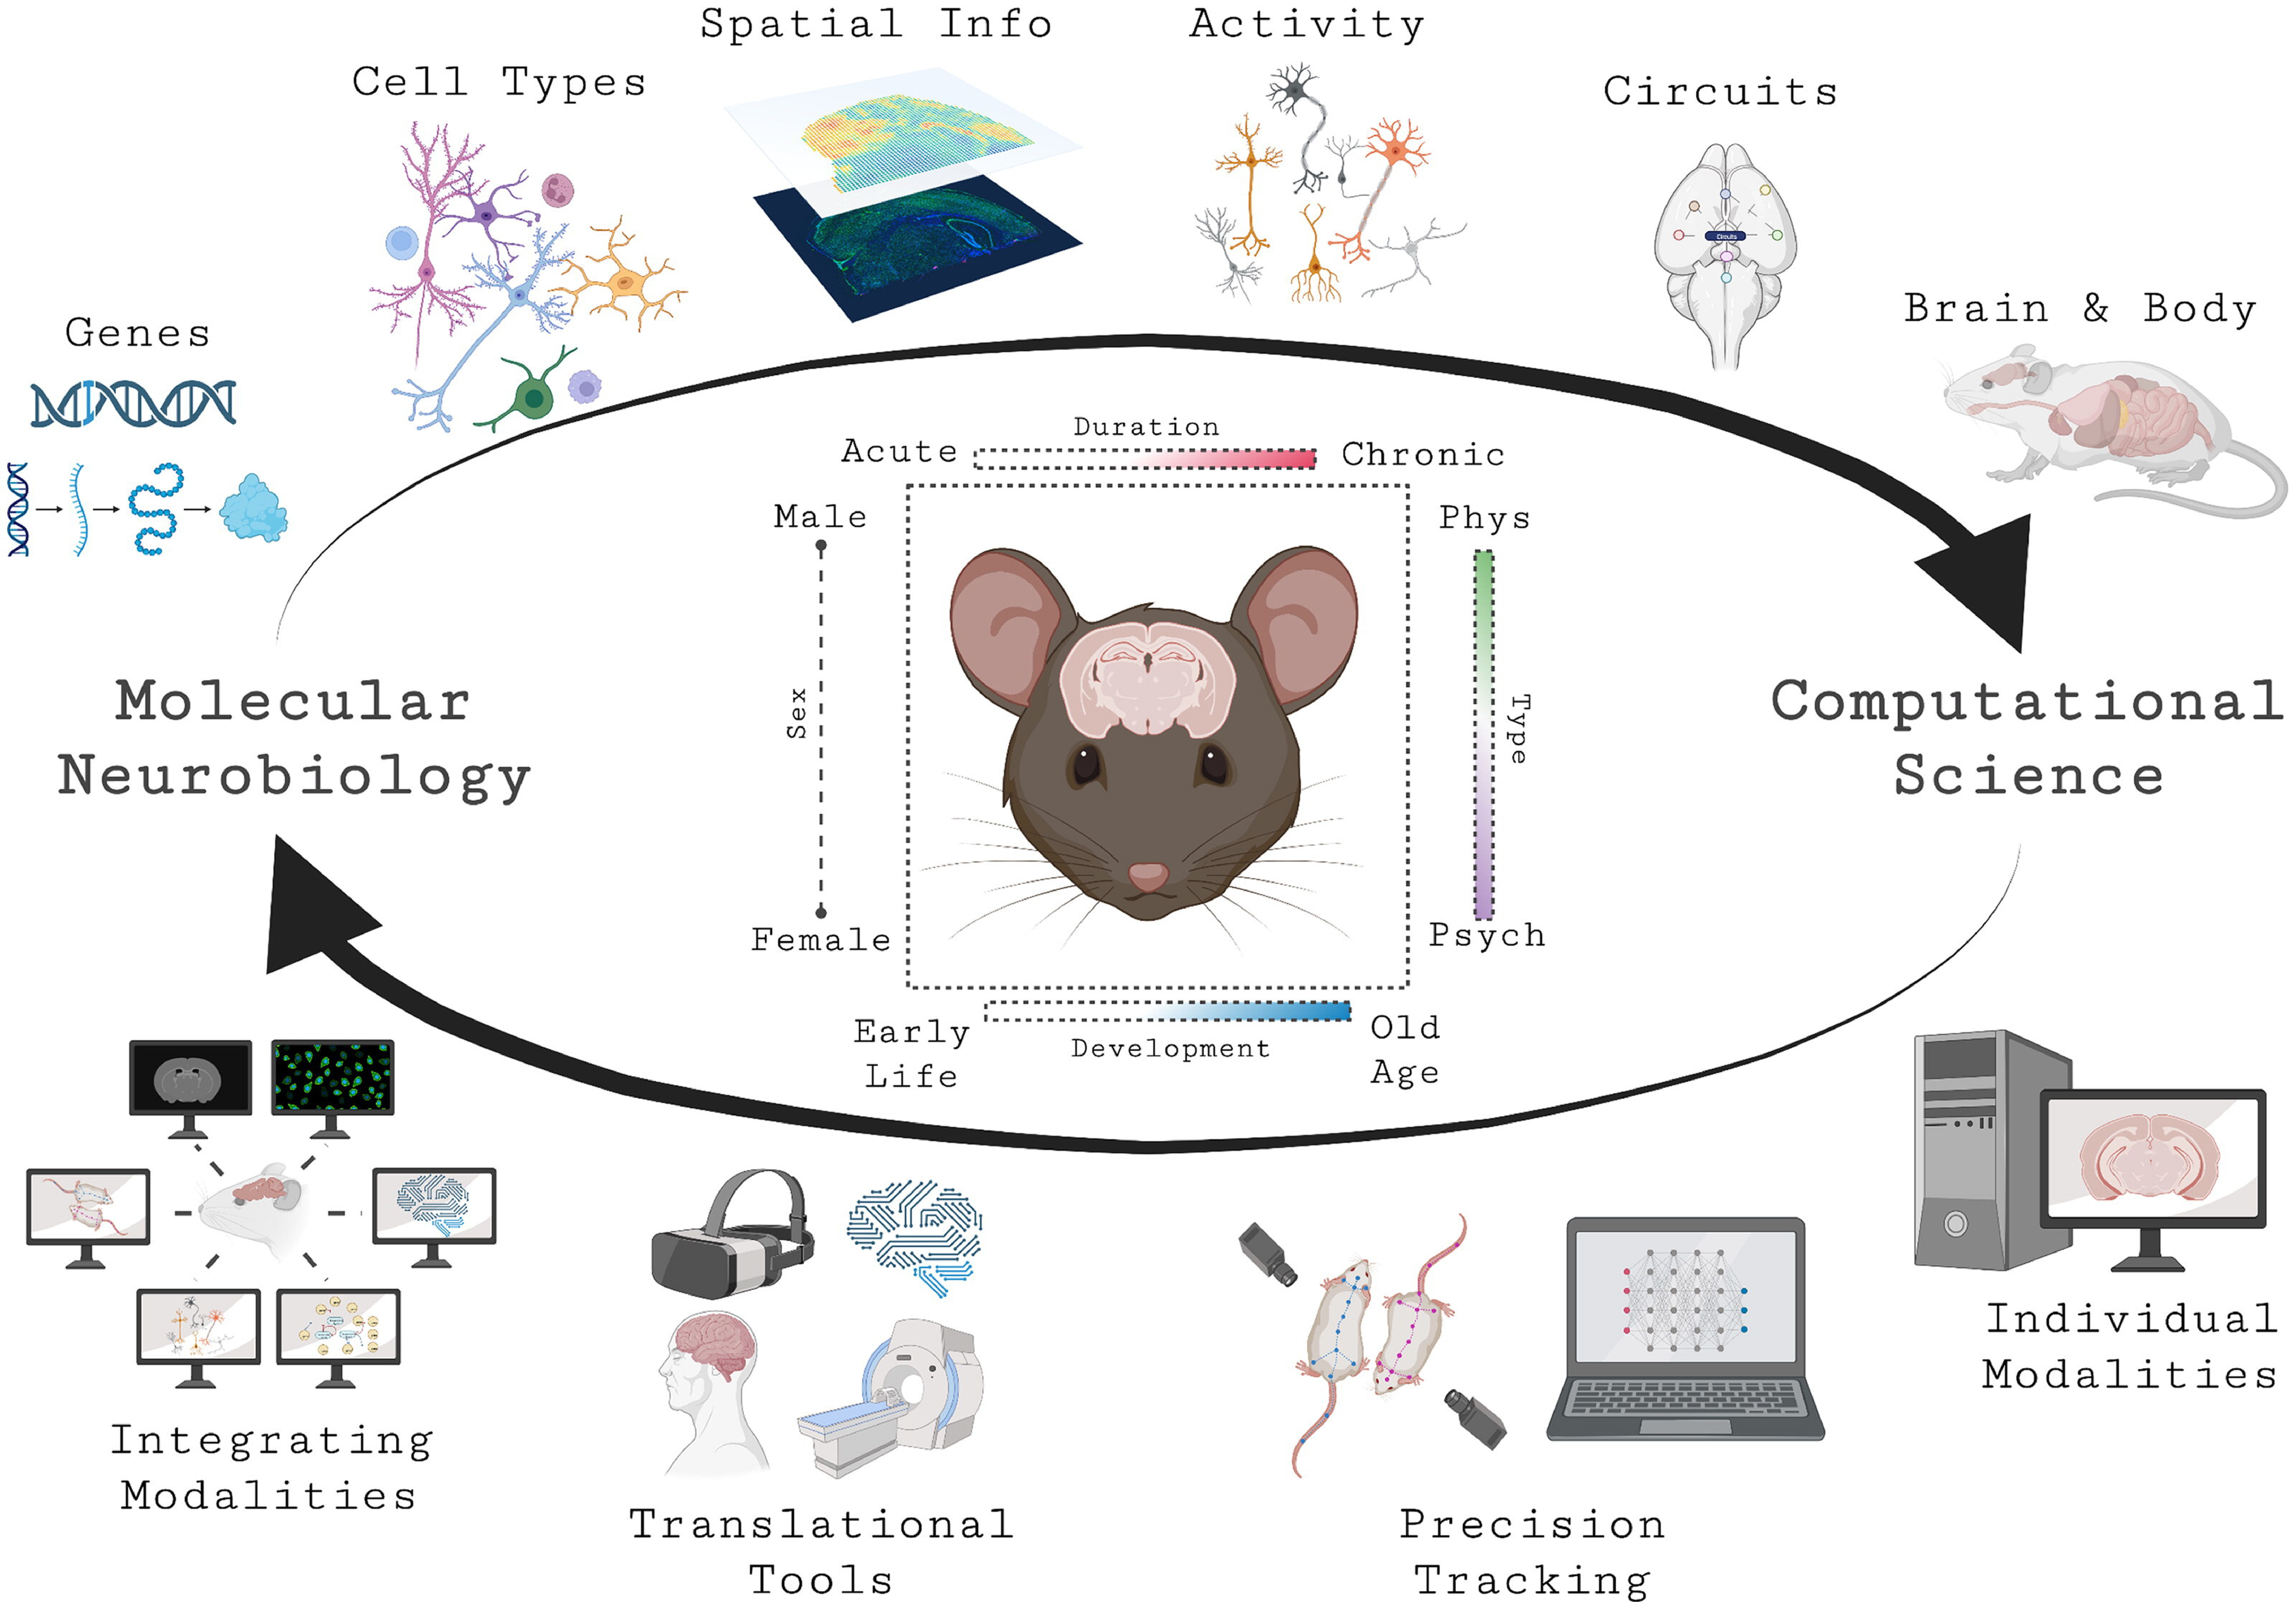
\includegraphics[width=\textwidth]{Figures/intro_6.pdf}

\caption[\textbf{From macro to micro: increasing resolution in stress neurobiology}]{\textbf{From macro to micro: increasing resolution in stress neurobiology.}  The field of stress neurobiology is benefiting from the increasing resolution offered by cutting-edge molecular and computational advancements. This focus on enhanced spatiotemporal resolution is affecting cell biology, behavioral science, and their interaction. The stress response can be studied from various perspectives, such as the nature of the stressor (physical versus psychological), the duration of the stressor (acute or chronic), the stage of development (from early life through adolescence, adulthood, and old age), or even the sex of the subject (male or female). (Created with BioRender.com, adapted from \cite{Miranda2023IncreasingBehaviors}).}
\label{fig:1.6}

\end{figure}

\subsection{Chronic Social Defeat Stress (CSDS)}

In this context, the CSDS paradigm is a widely used animal model, predominantly in rodents, for studying the effects of chronic stress on behavior and its potential contribution to the development of stress-related psychiatric disorders, such as MDD, anxiety disorder, and PTSD \cite{Russo2013TheDisorders}. The model aims to simulate territorial dominance, and involves repeated exposure to social stress through daily confrontations between a test subject, typically a mouse, and a more aggressive and dominant conspecific \cite{Golden2011AMice}. These encounters generally include physical aggression, which leads to subordination and submission in the test animal. Thus, and while far from perfect, the CSDS paradigm is designed to mimic aspects of chronic stress experienced by humans and induce behavioral, neurobiological, and physiological changes that resemble those observed in stress-related psychiatric conditions.

In most commonly used CSDS protocols, test animals undergo a series of daily stress exposures, usually lasting between 10 and 21 days \cite{Golden2011AMice}. After each confrontation with the conspecific, the test subject and the aggressor are housed in the same cage but separated by a mesh-like barrier, allowing continuous sensory contact while preventing further physical aggression. This continuous exposure to the stressor promotes the development of stress-related behaviors in the test animal, such as anhedonia, anxiety-like behavior, reduced motivation, and social avoidance \cite{Kudryavtseva1991SocialStrain, Iniguez2014SocialMice, Yoshida2021ChronicMice}. Following the chronic stress exposure, researchers typically assess these behaviors using various tests, aiming to quantify differences in social interaction and avoidance, sucrose preference, or locomotion (among others), to evaluate the effects of CSDS on the animal. Additionally, and in line with what was previously discussed about animal models, the CSDS paradigm enables the investigation of the underlying neurobiological and molecular mechanisms involved in stress-induced behavioral changes, as well as the evaluation of potential therapeutic interventions for stress-related disorders \cite{Donahue2014EffectsMice, Lopez2022KetamineKcnq2}.

\begin{figure}[!thb]
\centering
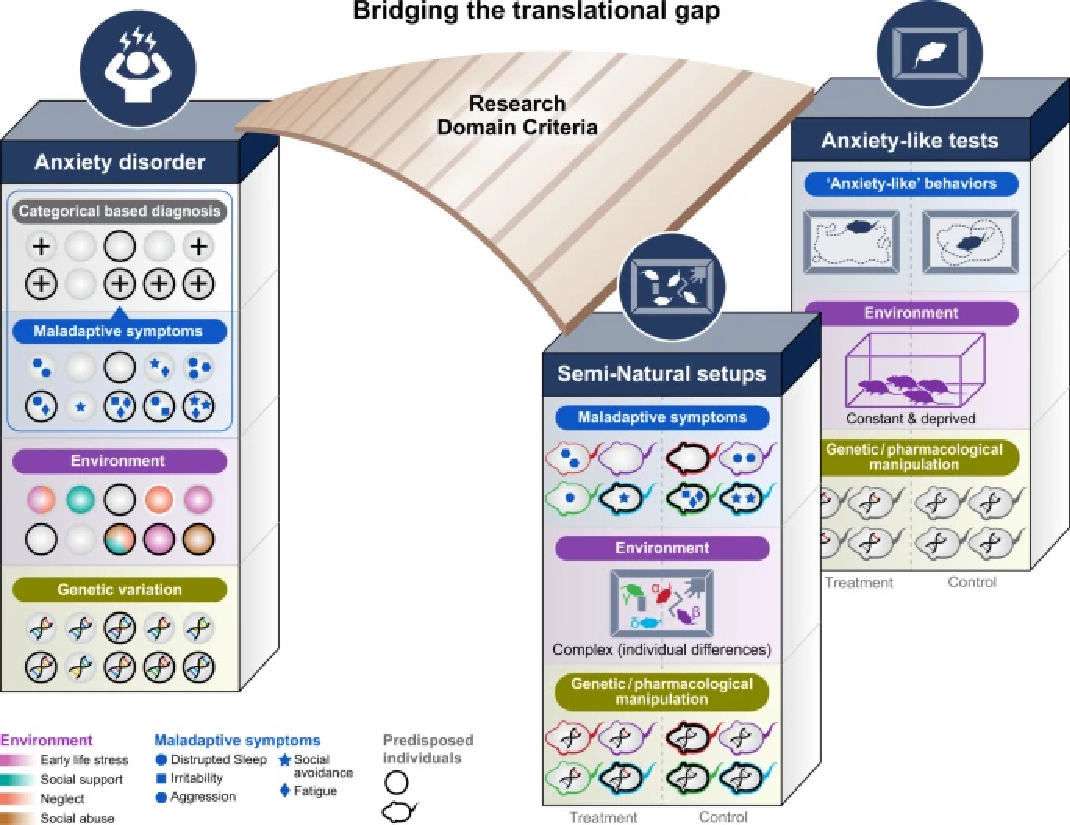
\includegraphics[width=\textwidth]{Figures/intro_7.pdf}

\caption[\textbf{A paradigm shift in translational psychiatry through rodent neuroethology}]{\textbf{A paradigm shift in translational psychiatry through rodent neuroethology:} So far, the use of animal models in the translational research of mental disorders hasn't managed to live up to the hopes of discovering new treatments. Human mental illnesses like anxiety disorders are complex, shaped by genetic factors, environmental influences past and present, and the interplay between these elements. In this context, disease diagnosis relies on categorized behavioral criteria (indicated in the figure by `+' symbols). In contrast, constructs like anxiety in mice are typically modeled using brief tests that identify `disease-like' phenotypes. Despite the high level of control, this behavioristic approach falls short in capturing the complexity of human mental illnesses. Automated tracking of complex behavior in mouse groups (in a semi-natural setup) can disclose individual coping mechanisms, so that the integration of univariate tests and semi-natural setups in the study of endophenotypes shared across mammalian species holds promise for narrowing this existing gap. (Adapted from \cite{Shemesh2023ANeuroethology}).}
\label{fig:1.7}

\end{figure}

While a widely adopted framework, however, the reduction of the overall shifts in behavior induced by this protocol can lead to an oversimplification of the associated behavioral repertoire, as well as to increasing the risk for cross-over effects with other types of behavior, such as anxiety. Moreover, due to technological limitations, the analysis of the interaction between multiple freely moving animals remained historically difficult, which further limited the complexity of the behavioral assessment \cite{Shemesh2023ANeuroethology}. Along these lines, social behavior is a complex entity that relies on many different types of behavioral interactions, which often are too complicated, time-intensive, and repetitive to assess manually \cite{Bordes2023AutomaticallyStress}. Ultimately, this makes CSDS an optimal scenario for the development of new tools, since any newly developed methods should recapitulate the available knowledge (which acts as a positive control) and room for improvement both in terms of throughput and behavioral insight is clear. As previously discussed, and while it remains impossible to fully replicate human disorders in animal models, the systematic development and thorough characterization of existing and new models can not only benefit basic research, but also help to bridge the overarching translational gap that exists in psychiatry today \cite{Shemesh2023ANeuroethology} (Figure~\ref{fig:1.7}).

In this context, this thesis aims to develop and present novel methods to analyze and describe behavior in experimental mice, deploy them at scale, and apply them to increase resolution in current descriptions of CSDS. Before addressing these goals, chapter \ref{chap:sota} will delve into the technical state of the art of the field.
